\documentclass[11pt]{article}
\usepackage{tikz}
\usetikzlibrary{arrows}
\usepackage{pgfmath}
\usepackage{setspace}
\usepackage{amsmath}
\usepackage{array}
\usepackage{hyperref}
\usepackage{enumerate}
\usepackage{enumitem}
\usepackage[normalem]{ulem}
\setlength{\pdfpageheight}{11in}
\setlength{\textheight}{9in}
\setlength{\voffset}{-1in}
\setlength{\oddsidemargin}{0pt}
\setlength{\marginparsep}{0pt}
\setlength{\marginparwidth}{0pt}
\setlength{\marginparpush}{0pt}
\setlength{\textwidth}{6.5in}

\pagestyle{empty}
%\setlength{}{}

\title{CSCE 515 Midterm Exam Prep}
\author{Brad Burkman}
\date{Last Edit: \today}

\begin{document}
\setlength{\parindent}{20pt}
\begin{spacing}{1.2}
\maketitle

\section{Checklist}

\begin{itemize}
	\item To Expand/Fix:  Exercise \#13, 20
	\item Done:  \#1, 2, 3,  4, 5, 6, 7, 8, 9, 11, 12, 14, 15, 16, 17, 18
\end{itemize}

\section{Topics to Solidify}

\begin{itemize}
	\item Lighting
	\item Perspective
\end{itemize}

\tableofcontents

%%%%%%%%%%%%%%%%%%
\section{Study Guide Questions}
%%%%%%%%%%%%%%%%%

%%%%%%%%%
\subsection{Question 1:  Refresh Buffers}
1.  Both raster and vector displays use a refresh buffer.  What is the difference between the two in terms of refresh buffer contents?

\subsubsection{First Punt, Brad Burkman, 11/17 7:41pm}

I have no idea.  I do not have a vector display refresh buffer in my notes, and I can't find it online.  

\

Here's what I do know.  

\

Raster displays have a bitmap of the color and intensity of each pixel.  Their refresh buffer holds the next screen to be displayed.  It may have two layers so that the swap between the displays doesn't happen in the middle of an update.  If it's a CRT monitor, it paints the pixels in rows, not following the contours of each object.  Raster displays have a constant refresh rate.  

\

Vector displays, like an oscilloscope, move a laser or electron beam over the screen following the contours of each object, drawing it smoothly.  It starts redrawing the screen after it has finished drawing the screen.  

\subsubsection{Marcus Shannon's Answer}

Q1: According to my class notes

\begin{itemize}
    \item Vector Display Refresh Buffers contain a series of commands directing how the electron gun is controlled by the deflection plates, organizing an effective way to draw lines onto the display.
    \item Raster Display Refresh Buffers contain a 2-dimensional bitmap/pixmap which is then used to render per-pixel data via the video controller onto the display.
\end{itemize}

\subsubsection{Brief Answer}

In a vector display, the refresh buffer contains instructions for drawing the page.  

In a raster display, the refresh buffer contains a pixmap of the page.  


%%%%%%%%%%%
\subsection{Question 2:  Besenham Algorithm}
2.  For the midpoint line algorithm, how were floating point operations converted to integer operations for the main loop?  (Be as specific as possible.)

\subsubsection{First guess, Brad Burkman, 11/14 7:44pm}
The floating point operations were multiplied by [something like] the number of pixels that each integer represented, then rounded, because we don't care about being between two pixels; we have to pick one.  

\subsubsection{Second Atttempt, informed by notes, Brad Burkman, 11/14 7:58pm}
Since this sample question is about a small piece of the Besenham algorithm, I presume the actual exam question could be anything about it.  

\

Looking at the notes from 28 August, here's how the midpoint (Besenham) algorithm works.

\subsubsection{Midpoint Line (Besenham) Algorithm}

\begin{tikzpicture}[x=40mm, y=40mm]
	\draw (0,0) -- (4,1.6);
	\draw (0,0) circle (5pt);
	\draw (1,0) circle (5pt);
	\draw (2,1) circle (5pt);
	\draw (3,1) circle (5pt);
	\fill (0,0) circle (2pt) node [below] {$(x_0,y_0)$};
	\fill (1,0) circle (2pt) node [below] {$(x_{1},y_0)$};
	\path (1,-0.2) node [below] {$=(x_{0}+1,y_{0})$};
	\path (1,-0.4) node [below] {$=(x_{1},y_{1})$};
	\fill (1,1) circle (2pt) node [above] {$(x_{1},y_1)$};
	\fill (1,0.4) circle (2pt) node [left] {$(x_{1}, y_0+m) \ $};
	\fill (1,0.5) circle (2pt) node [above left] {$(x_{1}, y_0+0.5) \ $};
	\fill (2,0) circle (2pt) node [below] {$(x_{2},y_{1})$};
	\fill (2,0.4) circle (2pt) node [below right] {$(x_{2},y_{0}+m)$};
	\fill (2,0.5) circle (2pt) node [above right] {$(x_{2}, y_0+0.5)$};
	\fill (2,0.8) circle (2pt) node [right] {$(x_{2},y_{0}+2m)$};
	\fill (2,1) circle (2pt) node [above] {$(x_{2},y_{0}+1)$};
	\path (2,1.2) node [above] {$=(x_{2},y_{2})$};
	\fill (3,1) circle (2pt) node [below right] {$(x_3,y_2)= (x_0+3,y_0+1)$};
	\fill (3,1.2) circle (2pt) node [right] {$(x_0+3,y_0+3m)$};
	\fill (3,1.5) circle (2pt) node [right] {$(x_0+3,y_0+1.5)$};
	\fill (3,2) circle (2pt) node [right] {$(x_0+3,y_0+2)$};
\end{tikzpicture}  

Initialize $d$ at $m - 0.5$.  

Since in this case $d$ is negative, choose to move E rather than NE.  

At the second step, because we moved E, $d = d+m$, so $d = 2m - 0.5$.  

Since $d$ is positive, move NE.  

Now since we moved NE, $d = d+m-1 = (2m-0.5) + m - 1 = 3m - 1.5$

Since $d = 3m-1.5$ is negative, move E.

\subsubsection{Making it Faster}

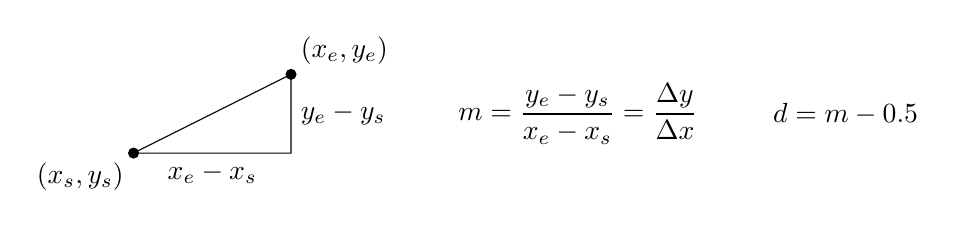
\begin{tikzpicture}[x=10mm,y=10mm]
	\draw (0,0) -- (2,1) -- (2,0) -- (0,0);
	\fill (0,0) circle (2pt) node [below left] {$(x_s,y_s)$};
	\fill (2,1) circle(2pt) node [above right] {$(x_e,y_e)$};
	\path (1,0) node [below] {$x_e-x_s$};
	\path (2,0.5) node [right] {$y_e - y_s$};
	\path (4,0.5) node [right] {$\displaystyle m = \frac{y_e - y_s}{x_e - x_s} = \frac{\Delta y}{\Delta x}$};
	\path (8,0.5) node [right] {$d = m-0.5$};
\end{tikzpicture}

Scale everything by $2 \Delta x$, so that $m = 2\Delta y$ and $d = 2\Delta y - \Delta x$.

\

Same example as above:

\begin{tikzpicture}[x=10mm,y=10mm]
	\draw (0,0) -- (5,2) -- (5,0) -- (0,0);
	\fill (0,0) circle (2pt) node [below left] {$(0,0)$};
	\fill (5,2) circle(2pt) node [above right] {$(5,2)$};
	\path (2.5,0) node [below] {$5$};
	\path (5,1) node [right] {$2$};
	\path (7,1) node [right] {$\displaystyle m = \frac{2}{5} = \frac{\Delta y}{\Delta x}$};
	\path (10,1) node [right] {$d = m-0.5$};
	\foreach \i in {0,1,2,3,4,5}{
		\draw [ultra thin, dashed] (\i,-1) -- (\i,3);
	}
\end{tikzpicture}

\

\begin{tikzpicture}[x=10mm,y=10mm]
	\draw (0,0) -- (5,2) -- (5,0) -- (0,0);
	\fill (0,0) circle (2pt) node [below left] {$(0,0)$};
	\fill (5,2) circle(2pt) node [above right] {$(50,20)$};
	\path (2.5,0) node [below] {$50$};
	\path (5,1) node [right] {$20$};
	\path (7,1) node [right] {$\displaystyle 2m\Delta x = 4 = \Delta y$};
	\path (7,0) node [right] {$d = 4-5 = -1$};
	\foreach \i in {0,1,2,3,4,5}{
		\draw [ultra thin, dashed] (\i,-1) -- (\i,3);
	}
\end{tikzpicture}

Initialize $d$ at $2\Delta y - \Delta x = 4-5 = -1$  

Since in this case $d$ is negative, choose to move E rather than NE.  

At the second step, because we moved E, $d = d+2\Delta y$, so $d = -1 + 4 = 3$.  

Since $d$ is positive, move NE.  

Now since we moved NE, $d = d+2 \Delta y - 10 = 3 + 2(2) - 10 = -3$

Since $d = -3$ is negative, move E.

\subsubsection{Brief Answer}

In the midpoint line (Besenham) algorithm, the floating point algorithm was adding some multiples of $m = \frac{\Delta y}{\Delta x}$ and $0.5$, so scale everything by $2\Delta x$ and you have integers.  

%%%%%%%%%%%%%%
\subsection{Question 3:  Vocabulary}
3.  What is meant by each of the three terms geometry, topology, and attributes for a polygonal surface model?

\subsubsection{Information from Class Notes, Brad Burkman, 17 November 10:11pm}

\begin{itemize}
	\item Vertex list gives the geometry, the shape.  
	\item Index list gives the topology, the relationships between neighbors.  
	\item Attributes are colors and normal vectors, perhaps the texture?
\end{itemize}

%%%%%%%%%%%%%
\subsection{Question 4:  Triangle Strips}

\sout{4.  Give an example of an operation that would normally be faster with pointers-to-a-vertex-list mesh representation than with an explicit representation.  Justify your answer.  }

Replace with:

Triangle Strips Question

\subsubsection{What kind of question could it be?}

\begin{itemize}
	\item Primitive restart index
	\item Vertices 0,1,2 define first triangle, 1,2,3 define second. 
	\item First triangle in the strip determines winding order.  Default is counterclockwise for the exterior, clockwise for the interior.  
	\item Given a rotated surface with $np$ number of points to be rotated and $nm$ steps of rotation, how many vertices, cells, triangles, triangles, triangle strips, elements in the vertex list, elements in the index list ... are there?
\end{itemize}

%%%%%%%%%%%%%%%%
\subsection{Question 5:  Transformations}
5.  Answer true or false for each item below.  

For transforms as discussed in class:

\begin{itemize}
	\item Any two rotations are commutative.
	
	False.  See example below. 
	\item Any two translations are commutative.
	
	True.
	\item The inverse of a rotation matrix is its transpose.  
	
	True
	\item The inverse of a translation matrix is its transpose.  
	
	False
	\item For any composite sequence of translations and rotations, there exists a single rotation and translation pair that would have the same net effect.  [Dr. Borst says it's true.]
\end{itemize}

\subsubsection{Rotation Matrices}

What do we know about rotation matrices?

\begin{itemize}
	\item Each row, and each column, is a unit vector, because we're not changing scale.
	\item The determinant of the matrix is 1.
	\item They are orthogonal; {\tt i.e.} $R^{-1} = R^T$.
\end{itemize}

\subsubsection{$Z$-rotation matrix}

$$
\left[
\begin{array}{cccc}
	\cos \theta & - \sin \theta & 0 & 0 \cr
	\sin \theta & \cos \theta & 0 & 0 \cr
	0 & 0 & 1 & 0 \cr
	0 & 0 & 0 & 1 \cr
\end{array}
\right]
$$

\subsubsection{$Y$-rotation matrix}

$$
\left[
\begin{array}{cccc}
	\cos \theta & 0 & \sin \theta & 0 \cr
	0 & 1 & 0 & 0 \cr
	-\sin \theta & 0  & \cos \theta & 0 \cr
	0 & 0 & 0 & 1 \cr
\end{array}
\right]
$$

\subsubsection{$X$-rotation matrix}

$$
\left[
\begin{array}{cccc}
	1 & 0 & 0 & 0 \cr
	0 & \cos \theta & -\sin \theta & 0 \cr
	0 & \sin \theta & \cos \theta & 0 \cr
	0 & 0 & 0 & 1 \cr
\end{array}
\right]
$$

Let's multiply two of them together and see whether it's commutative.  

$$YX = 
\left[
\begin{array}{cccc}
	\cos \beta & 0 & \sin \beta & 0 \cr
	0 & 1 & 0 & 0 \cr
	-\sin \beta & 0  & \cos \beta & 0 \cr
	0 & 0 & 0 & 1 \cr
\end{array}
\right]
\left[
\begin{array}{cccc}
	1 & 0 & 0 & 0 \cr
	0 & \cos \alpha & -\sin \alpha & 0 \cr
	0 & \sin \alpha & \cos \alpha & 0 \cr
	0 & 0 & 0 & 1 \cr
\end{array}
\right]
=\left[
\begin{array}{cccc}
	\cos \beta & \sin \alpha \sin \beta & \cos \alpha \sin \beta & 0 \cr
	0 & \cos \alpha & -\sin \alpha & 0 \cr
	-\sin \beta & \sin \alpha \cos \beta & \cos \alpha \cos \beta & 0 \cr
	0 & 0 & 0 & 1 \cr
\end{array}
\right]
$$

$$XY = 
\left[
\begin{array}{cccc}
	1 & 0 & 0 & 0 \cr
	0 & \cos \alpha & -\sin \alpha & 0 \cr
	0 & \sin \alpha & \cos \alpha & 0 \cr
	0 & 0 & 0 & 1 \cr
\end{array}
\right]
\left[
\begin{array}{cccc}
	\cos \beta & 0 & \sin \beta & 0 \cr
	0 & 1 & 0 & 0 \cr
	-\sin \beta & 0  & \cos \beta & 0 \cr
	0 & 0 & 0 & 1 \cr
\end{array}
\right]
=\left[
\begin{array}{cccc}
	\cos \beta & 0 & \sin \beta & 0 \cr
	\sin \alpha \sin \beta & \cos \alpha & -\sin \alpha \cos \beta & 0 \cr
	-\cos \alpha \sin \beta & \sin \alpha & \cos \alpha \cos \beta & 0 \cr
	0 & 0 & 0 & 1 \cr
\end{array}
\right]
$$


%%%%%%%%%%%%%%%%%%
\subsection{Question 6:  Composite Homogeneous Transform}
6.  Give a $4 \times 4$ homogeneous transform (sixteen numbers) for describing an object's local coordinate system with respect to the world coordinate system such that:

\begin{itemize}
	\item The object's local origin is at world coordinate $(x,y,z) = (4,0,2)$,
	\item The object's local $x$-axis direction matches the world's $z$-axis direction, and 
	\item The object's local $z$-axis direction matches the world's $-x$ (negative $x$) direction, 
\end{itemize}

\subsubsection{Brad's answer, 18 November 6:44 am}

A $-90^{\circ}$ rotation in the $Y$ gives the correct orientation. 

Do the rotation, then the translation.  

$$A = T_{(4,0,2)} Y_{-90} = 
\left[
\begin{array}{cccc}
	1 & 0 & 0 & 4 \cr
	0 & 1 & 0 & 0 \cr
	0 & 0 & 1 & 2 \cr
	0 & 0 & 0 & 1 \cr
\end{array}
\right]
\left[
	\begin{array}{cccc}
		\cos (-90) & 0 & \sin (-90) & 0 \cr
		0 & 1 & 0 & 0 \cr
		-\sin(-90) & 0 & \cos (-90) & 0 \cr
		0 & 0 & 0 & 1 \cr
	\end{array}
\right]
$$

$$= 
\left[
\begin{array}{cccc}
	1 & 0 & 0 & 4 \cr
	0 & 1 & 0 & 0 \cr
	0 & 0 & 1 & 2 \cr
	0 & 0 & 0 & 1 \cr
\end{array}
\right]
\left[
	\begin{array}{cccc}
		0 & 0 & -1 & 0 \cr
		0 & 1 & 0 & 0 \cr
		1 & 0 & 0 & 0 \cr
		0 & 0 & 0 & 1 \cr
	\end{array}
\right]
$$

$$= 
\left[
	\begin{array}{cccc}
		0 & 0 & -1 & 4 \cr
		0 & 1 & 0 & 0 \cr
		1 & 0 & 0 & 2 \cr
		0 & 0 & 0 & 1 \cr
	\end{array}
\right]
$$

%%%%%%%%%%%%%%%%
\subsection{Question 7:  Inverse Transform}

Give the inverse of the transform.  

$$A^{-1}= \left(T_{(4,0,2)} Y_{-90}\right)^{-1} = 
\left( Y_{-90} \right)^{-1}\left( T_{(4,0,2)}\right)^{-1} = 
Y_{90} T_{(-4,0,-2)}
$$

$$
\left[
	\begin{array}{cccc}
		\cos (90) & 0 & \sin (90) & 0 \cr
		0 & 1 & 0 & 0 \cr
		-\sin(90) & 0 & \cos (90) & 0 \cr
		0 & 0 & 0 & 1 \cr
	\end{array}
\right]
\left[
\begin{array}{cccc}
	1 & 0 & 0 & -4 \cr
	0 & 1 & 0 & 0 \cr
	0 & 0 & 1 & -2 \cr
	0 & 0 & 0 & 1 \cr
\end{array}
\right]
$$

$$= 
\left[
	\begin{array}{cccc}
		0 & 0 & 1 & 0 \cr
		0 & 1 & 0 & 0 \cr
		-1 & 0 & 0 & 0 \cr
		0 & 0 & 0 & 1 \cr
	\end{array}
\right]
\left[
\begin{array}{cccc}
	1 & 0 & 0 & -4 \cr
	0 & 1 & 0 & 0 \cr
	0 & 0 & 1 & -2 \cr
	0 & 0 & 0 & 1 \cr
\end{array}
\right]
$$

$$= 
\left[
	\begin{array}{cccc}
		0 & 0 & 1 & -2 \cr
		0 & 1 & 0 & 0 \cr
		-1 & 0 & 0 & 4 \cr
		0 & 0 & 0 & 1 \cr
	\end{array}
\right]
$$

Check.  

$$ A A^{-1} = \left[
	\begin{array}{cccc}
		0 & 0 & -1 & 4 \cr
		0 & 1 & 0 & 0 \cr
		1 & 0 & 0 & 2 \cr
		0 & 0 & 0 & 1 \cr
	\end{array}
\right]
\left[
	\begin{array}{cccc}
		0 & 0 & 1 & -2 \cr
		0 & 1 & 0 & 0 \cr
		-1 & 0 & 0 & 4 \cr
		0 & 0 & 0 & 1 \cr
	\end{array}
\right]
=
\left[
	\begin{array}{cccc}
		1 & 0 & 0 & 0 \cr
		0 & 1 & 0 & 0 \cr
		0 & 0 & 1 & 0 \cr
		0 & 0 & 0 & 1 \cr
	\end{array}
\right]
\qquad \surd
$$


%%%%%%%%%%%%%%%%%
\subsection{Question 8:  Unit Normal Vector}
8.  The diagrams below show a house model.  Give $\hat{\mathbf{n}}$, the unit normal vector for the right side of the roof.  

\subsubsection{First guess for \#8, Brad Burkman, 7:58pm, 11 November}
$$\hat{\mathbf{n}} = 
\left[
\begin{array}{>{\displaystyle}c<{\vrule width 0pt height 24pt depth 8pt}}
	 \frac{\sqrt2}{2}\cr
	 \frac{\sqrt2}{2}\cr
	 0 
\end{array}
\right]
$$

\subsubsection{Dr. Borst's Discussion}

Create a coordinate system, make a triangle, and use the cross product to find the normal.  

Front left top corner of the house at $A(1,1,1)$,

Back left top corner of the house at $B(1,1,-1)$,

Front peak of house at $\displaystyle C\left( 0,2, 1\right)$

Vector $\vec{u}$ from A to B: $\vec{u} = (0,0,-2)$

Vector $\vec{v}$ from A to C:  $\displaystyle\vec{v} = \left( -1,1, 0 \right)$

$\displaystyle
\vec{u} \times \vec{v} = {\mathbf{n}} = 
\left|
	\begin{array}{ccc}
		\vec{i} & \vec{j} & \vec{k} \cr
		0 & 0 & -2 \cr
		-1 & 1 & 0 \cr
	\end{array}
\right|
= 2\vec{i}  +2\vec{j} + 0\vec{k}
$

$\displaystyle
\hat{\mathbf{n}} = 
\frac{\mathbf{n}}{|\mathbf{n}|}
= \frac{2\vec{i} + 2 \vec{j} + 0 \vec{k}}{2\sqrt2} = \frac{\sqrt2}{2}\vec{i} + \frac{\sqrt2}{2} \vec{j} + 0 \vec{k}
=
\left[
	\begin{array}{>{\displaystyle\vrule width 0pt height 16pt depth 12pt}c}
		\frac{\sqrt2}{2} \cr
		\frac{\sqrt2}{2} \cr
		0 \cr
	\end{array}
\right]
$

%%%%%%%%%%%%%%%%
\subsection{Question 9:  Fixed Axis Angle / Euler Rotations}
9.  Recall the plane diagram above.  Suppose plane orientation is stored as an $X-Z-Y$ fixed axis set $(\theta, \phi, \alpha)$, that is, three rotations about fixed world axes in the order $X$, $Z$, $Y$.  In terms of the composite rotation resulting from these three components and for arbitrary plane orientation:

\begin{enumerate}[label=\arabic*)]
	\item A small change in $\theta$ ($X$ amount) will always cause rotation about:
	
	local $x_p$ \qquad local $y_p$ \qquad local $z_p$ \qquad world $x$ \qquad world $y$ \qquad world $z$ \qquad NOTA
	\item A small change in $\phi$ ($Z$ amount) will always cause rotation about:
	
	local $x_p$ \qquad local $y_p$ \qquad local $z_p$ \qquad world $x$ \qquad world $y$ \qquad world $z$ \qquad NOTA
	
	\item A small change in $\alpha$ ($Y$ amount) will always cause rotation about:
	
	local $x_p$ \qquad local $y_p$ \qquad local $z_p$ \qquad world $x$ \qquad world $y$ \qquad world $z$ \qquad NOTA
	\item If each component rotation is expressed as a matrix and then all three are composed into a single rotation matrix, the multiplication order for this representation would be:
	
	$R_XR_ZR_Y$ \qquad
	$R_YR_ZR_X$ \qquad
	$R_XR_YR_Z$ \qquad
	$R_ZR_YR_X$ \qquad
	NOTA
\end{enumerate}


\subsubsection{Marcus Shannon's Answer}
Q9: According to my class notes

\begin{itemize}
	\item Fixed - Axis Angles are guaranteed a single world rotation and a single local rotation. Everything else is considered questionable.

      For example: for the fixed axis angle set X, Z, Y ; X would be the world rotation and Y would be the local rotation. Z is considered questionable and no guarantees can be made about it's axis of rotation in relation to what coordinate system.
    \item Fixed Axis Angle rotations are calculated right to left, for XZY you'll get Y * Z * X.
    \item Euler Angle rotations are calculated left to right, for XYZ you'll get X * Y * Z.
\end{itemize}

%%%%%%%%%%%%%%%%%%%
\subsection{Question 10:  Quaternion}
10.  How could we convert an orientation expressed in a 3-angle set convention above to a single quaternion representing the same orientation?  Give a concise but accurate conceptual description.

\subsubsection{Dr. Borst's Answer}

``Convert each of the three components into a quaternion, and multiply them.'' [Dr. Borst]

$X-Z-Y$ fixed axis set is multiplied as $R_YR_ZR_X$.

\subsubsection{Marcus Shannon's Answer}
Q10: From deduction and expanding on Dr. Borst explanation of  "Convert each of the three components into a quaternion, and multiply them":

\begin{itemize}
    \item To start, we have a fixed axis angle set of XZY.
    \item Take each rotation and convert it into three separate Angle-Axis rotations:
    
        $ X \to x_\theta, u_x =  \left[ \begin{array}{c} 1\cr 0\cr 0\cr\end{array} \right]$\qquad
        $ Z \to z_\alpha, u_z =  \left[ \begin{array}{c} 0\cr 0\cr 1\cr\end{array} \right]$\qquad
        $ Y \to y_\phi u_y =  \left[ \begin{array}{c} 0\cr 1\cr 0\cr\end{array} \right]$
        
    	\item We then compute these using the conversion formula provided in class for converting Angle Axis form into Quaternion form:
        $$q = \cos(\theta/2) + (i)(u_x)(\sin(\theta/2)) + (j)(u_y)(\sin(\theta/2)) + (k)(u_z)(\sin(\theta/2))$$
    \item Composing these 3 quaternions, we now have a single quaternion composed of all rotations.
        $$q_{final} = qx * qz * qy$$
    \item Note: I don't claim for this to be the full expansion or correct, this is merely logical meandering based on what I currently understand.
    \end{itemize}
    
%%%%%%%%%%%%%%%%%
\subsection{Question 11:  Sequence of Transforms from Camera (Eye) to Object}
11.  The graph below represents the relationships between coordinate systems (objects, if you prefer) using notation from lecture.  Suppose $\{D\}$ is the camera's local frame in an OpenGL application.  When rendering an object having vertices described in frame $\{E\}$, what would the value of the modelview matrix be?

\subsubsection{First Guess, Brad Burkman, 8:26pm 14 November}

$$
	^D_CT \cdot 
	^C_AT \cdot 
	^A_BT \cdot 
	^B_ET = 
	\left( ^C_DT \right)^{-1} \cdot
	\left( ^A_CT \right)^{-1} \cdot
	^A_BT \cdot 
	^B_ET
	$$

%%%%%%%%%%%%%%%%%
\subsection{Question 12:  Local/Global Transform}
12.  Suppose, for the above diagram, we want to rotate frame $\{B\}$ by a rotation transform $R$ that is to act as a rotation described with respect to the  current $\{B\}$ frame.  How exactly should $R$ be applied to update one of the transforms in the graph?

\subsubsection{Dr. Borst's Answer}

$^A_BT$ gets modified.  Multiply by $R$ on the right to be a local change to $B$.  

%%%%%%%%%%%%%%%%%%%%%%%%
\subsection{Question 13:  Perspective Projection Matrices}
13.  Give any one of the perspective projection matrices, $M_{per}$ from the lecture slides.  

\subsubsection{Orthographic Projection from Simple Example}

$$M_{ort} = 
\left[
	\begin{array}{cccc}
		1 & 0 & 0 & 0 \cr
		0 & 1 & 0 & 0 \cr
		0 & 0 & 0 & 0 \cr
		0 & 0 & 0 & 1 \cr
	\end{array}
\right]
$$

\subsubsection{Extended Orthographic Projection Matrix}

$$M_{ort,norm} = 
\left[
	\begin{array}{cccc}
		1 & 0 & 0 & 0 \cr
		0 & 1 & 0 & 0 \cr
		0 & 0 & -1 & 0 \cr
		0 & 0 & 0 & 1 \cr
	\end{array}
\right]
\left[
	\begin{array}{cccc}
		\frac{2}{r-l} & 0 & 0 & 0 \cr
		0 & \frac{2}{t-b} & 0 & 0 \cr
		0 & 0 & \frac{2}{f-n} & 0 \cr
		0 & 0 & 0 & 1 \cr
	\end{array}
\right]
\left[
	\begin{array}{cccc}
		1 & 0 & 0  & -\frac{l+r}{2} \cr
		0 & 1 & 0 & -\frac{b+t}{2} \cr
		0 & 0 & 1 & \frac{n+f}{2} \cr
		0 & 0 & 0 & 1 \cr
	\end{array}
\right]
$$

\subsubsection{Perspective Matrix}

Basic perspective matrix.  


$$
\left[
	\begin{array}{cccc}
		X \cr
		Y \cr
		Z \cr
		W \cr
	\end{array}
\right]
=
M_{per} \cdot p = 
\left[
	\begin{array}{cccc}
		-n & 0 & 0 & 0 \cr
		0 & -n & 0 & 0 \cr
		0 & 0 & -n & 0 \cr
		0 & 0 & 1 & 0 \cr
	\end{array}
\right]
\left[
	\begin{array}{cccc}
		x \cr y \cr z \cr 1
	\end{array}
\right]
= 
\left[
	\begin{array}{cccc}
		-nx \cr -ny \cr -nz \cr z
	\end{array}
\right]
=
\left[
	\begin{array}{cccc}
		-nx/z \cr -ny/z \cr -n & 1 \cr
	\end{array}
\right]
=
\left[
	\begin{array}{cccc}
		x_p \cr y_p \cr z_p \cr 1 \cr
	\end{array}
\right]
$$

Generalized perspective matrix

$$
M_{per} = 
\left[
	\begin{array}{cccc}
		-n & 0 & 0 & 0 \cr
		0 & -n & 0 & 0 \cr
		0 & 0 & -(n+f) & -nf \cr
		0 & 0 & 1 & 0 \cr
	\end{array}
\right]
$$

Preserves some depth info ($z$ coordinate)

$Z$-coordinate is unchanged at near and far boundaries

Transforms the frustum into an orthographic view volume.  

%%%%%%%%%%%%%%%%%%
\subsection{Question 14:  Normalizing Transform}
14.  What is meant by a normalizing transform and what two substeps can be used to build the normalizing transform for the orthographic projection case described in lecture?  A good conceptual description is sufficient; exact transforms are not requested.

\subsubsection{Dr. Borst's Answer}

Normalizing transform takes a box in the view and transforms it to $[-1,1]\times [-1,1] \times [-1,1]$.  Transform the center to the origin and scale.  

%%%%%%%%%%%%%%%%%
\subsection{Question 15:  Modelview Matrix (Definition)}
15.  In the OpenGL pipeline, after the modelview matrix is applied to a vertex, the result is that the vertex is described with respect to which coordinate system?

\

ModelView Matrix is the composition of all of the transformations from the camera to the
node being rendered.

\ 

Answer:  Camera View
\subsubsection{Note from Marcus Shannon for \#15 and \#16}
Q15 \& Q16: This is a trivial point to make but the Camera View, from my understanding, is equivalent to the Eye Coordinate System.

%%%%%%%%%%%%%%%%
\subsection{Question 16:  Perspective Frustum}
16.  The six common parameters (near, far, left, $\dots$) of a perspective frustum description are coordinates describing the viewing volume with respect to which coordinate system?

\

Answer:  Camera View

\subsubsection{First Guess, Brad Burkman, 9:03pm 14 November}

Eye (camera) coordinate system.

%%%%%%%%%%%%%%%%%
\subsection{Question 17:  Illumination Equation}
17.  Below, circle all correct answers for questions about the illumination equation from lecture.  

\begin{enumerate}[label=\arabic*)]
	\item Which of the following vectors is (are) used in computing the ambient lighting term?
	
	Direction to light \qquad Surface normal \qquad Direction to viewer \qquad None
	\item Which of the following vectors is (are) used in computing the diffuse lighting term?
	
	Direction to light \qquad Surface normal \qquad Direction to viewer \qquad None
	\item Which of the following vectors is (are) used in computing the specular lighting term?
		
	Direction to light \qquad Surface normal \qquad Direction to viewer \qquad None

\end{enumerate}

\subsubsection{Marcus Shannon's Answer}

Q17: This is simply about looking at the Phong Illumination Equation and identifying what vectors come into play with what parts.
\begin{itemize}
    \item Ambient light only considers: Reflection Coefficient (Ka), Ambient Light Intensity (Ia), \& RGB of Object (Od).  
      \item Therefore 1) is None.
    \item Diffuse considers: Diffuse Coefficient (Kd), Diffuse Light Intensity (Id), Normalized Light Normal (N with hat), \& Normalized Light Direction (L with hat).
      \item Therefore 2) is Direction to light \& Surface Normal.
    \item Specular considers: Specular Coefficient (Ks), Specular Object (Os), Specular Exponent (n), Normalized Reflection (R with hat), \& Direction to Viewer (V with hat).
      \item Initially, it looks as though the answer is the same as 2) however R (with hat) expands into using N (with hat) \& L (with hat).
      \item Therefore 3) is Direction to light, Surface Normal, \& Direction to Viewer.
\end{itemize}

\subsubsection{Lighting Equation}

\begin{tikzpicture}[x=30mm,y=30mm]
	\clip (-2,-.5) rectangle (2,1.5);
	\draw (0,-1) circle (1);
	\draw [-triangle 60] (0,0) -- ({cos(90)},{sin(90)}) node [above] {$\vec{N}$}; 
	\draw [-triangle 60] (0,0) -- ({cos(60)},{sin(60)}) node [above] {$\vec{R}$};  
	\draw [-triangle 60] (0,0) -- ({cos(120)},{sin(120)}) node [above] {$\vec{L}$}; 
	\draw [-triangle 60] (0,0) -- ({cos(20)},{sin(20)}) node [above] {$\vec{V}$}; 
	\draw ({0.5*cos(90)},{0.5*sin(90)}) arc (90:120:0.5) node [midway, above] {$\theta$};
	\draw ({0.4*cos(60)},{0.4*sin(60)}) arc (60:90:0.4) node [midway, above] {$\theta$};
	\draw ({0.5*cos(20)},{0.5*sin(20)}) arc (20:60:0.5) node [midway, above right] {$\phi$};
\end{tikzpicture}

{\bf Ambient Component}  $I = k_a I_a O_a$

$k_a \in [0,1]$ is the reflective coefficient, proportion of incident light reflected.  Usually a property of the material.

$I_a \in [0,1]$ is ambient light intensity

$O_a$ ambient color term

\

\noindent{\bf Diffuse Component}:  Which way is the surface facing?

$k_d$ object's diffuse-reflection coefficient

$I_l$ Light source intensity

$O_d$ Diffuse color term

$\hat{\mathbf{N}}$ Surface unit normal

$\hat{\mathbf{L}}$ Unit vector towards light

$\theta$ Angle between surface normal and direction towards light

$$I = k_d I_l O_d \cos \theta = k_d I_l O_d \left( \hat{\mathbf{N}} \cdot \hat{\mathbf{L}} \right)$$

\

\noindent {\bf Specular Component}:  Sharp reflections

$k_s$ Specular reflection coefficient

$I_l$ Light intensity

$O_s$ Object's specular color

$\phi$ Angle between reflection and viewer.  

Note:  If $\phi = 0$, then it's reflecting right into the eye view.  

$n$ Specular exponent.  The higher the $n$, the sharper the more narrow the reflection.  

$$I = k_s I_l O_s \cos^n \phi = k_s I_l O_s \left(\hat{\mathbf{R}} \cdot \hat{\mathbf{V}}\right) ^n$$


$$ I = k_a I_a O_a + k_d I_l O_l \cos \theta + k_s I_l O_s \cos^n \phi$$

$$\cos \theta = \hat{\mathbf{N}} \cdot \hat{\mathbf{L}}, \qquad 
\cos \phi = \hat{\mathbf{R}} \cdot \hat{\mathbf{V}}$$

$$ I = k_a I_a O_a + k_d I_l O_l \hat{\mathbf{N}} \cdot \hat{\mathbf{L}} + k_s I_l O_s \left(\hat{\mathbf{R}} \cdot \hat{\mathbf{V}}\right)^n$$

%%%%%%%%%%%%%%%%%
\subsection{Question 18: Phong/Gouraud Shading}
18.  Describe why a triangle may look different with Phong shading than with Gouraud shading, and include a sketch of shaded triangles that illustrate the difference you discuss. 

\subsubsection{Marcus Shannon's Solution}

Q18: Pulled from the slides (paraphrased):
\begin{itemize}
    \item Gourand shading will evaluate at polygon vertices \& interpolate resulting color across the polygon.
    \item Phong shading will interpolate surface normals from vertices \& then apply lighting equation per-pixel.
    \item For triangle shading, review the second set of slides provided on moodle and scroll down a bit.
\end{itemize}

\subsubsection{Brad's Solution (Same idea, expressed slightly differently)}

In Gouraud shading, the lighting equation is calculated at vertices and interpolated across the polygon to get values at each pixel.  

In Phong shading, the lighting equation is calculated at each pixel.  

Gouraud shading will be much smoother, with no spots of intensity.  

Phong shading, especially with strong diffuse and specular coefficients will have much sharper ``highlights.''  

%%%%%%%%%%%%%%%%%%
\subsection{Question 19:  Painter's Algorithm}
\sout{19.  Sketch a scene with two or three polygons for which the painter's algorithm would be insufficient for visible surface determination.  }

%%%%%%%%%%%%%%%%%%
\subsection{Question 20:  Scan Conversion}
20.  Consider scan conversion of the illustrated triangle.  Assume that scan conversion is done from the bottom up, that the triangle crosses several scan lines, and that the geometry matches the illustration.  

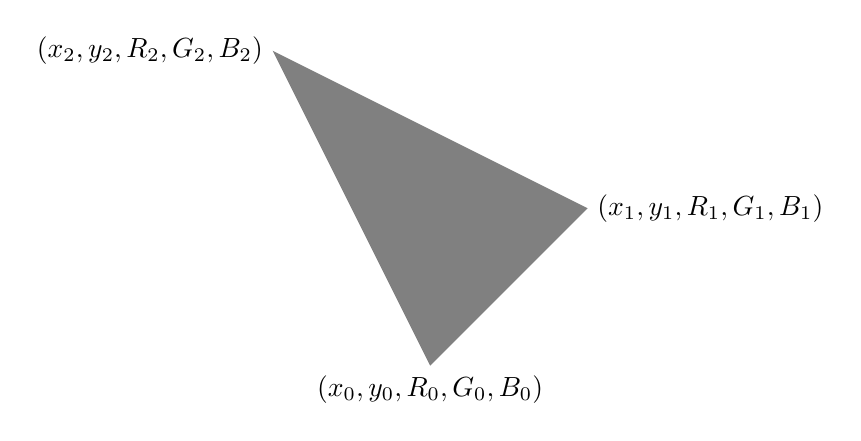
\begin{tikzpicture}[x=20mm,y=20mm]
	\coordinate (A) at (0,0);
	\coordinate (B) at (1,1);
	\coordinate (C) at (-1,2);
	\fill [gray] (A) -- (B) -- (C) -- (A);
	\path (A) node [below] {$(x_0, y_0, R_0, G_0, B_0)$};
	\path (B) node [right] {$(x_1,y_1,R_1,G_1,B_1)$};
	\path (C) node [left] {$(x_2,y_2,R_2,G_2,B_2)$};
\end{tikzpicture}

\begin{enumerate}[label=\arabic*)]
	\item In terms of the vertex coordinates and colors labeled on the diagram, give the coordinates and RGB color values for the first pixel to be colored.  
	\item In terms of the vertex coordinates and colors labeled on the diagram, give the coordinates and RGB values for the second pixel to be colored.  
\end{enumerate}

\subsubsection{First Guess, Brad Burkman, 9:23pm 14 November}

First pixel to be colored is the bottom.  
$$(x_0, y_0, R_0, G_0, B_0)$$

Second pixel to be colored is above left of that.  

$$m = \frac{y_2 - y_0}{x_2 - x_0} = \frac{\Delta y}{\Delta x}$$

Since we're going up one pixel, $\Delta y = 1$, so we're interested in $\Delta x$.  

$$\Delta x = \frac{x_2 - x_0}{y_2 - y_0}$$

and we're going to round it up (on the left, down on the right), because we're talking about pixel values, which are integers.  

$$\Delta x = \left\lceil\frac{x_2 - x_0}{y_2 - y_0}\right\rceil$$

Change in colors works the same way.  

$$\Delta R = \frac{R_2 - R_0}{y_2 - y_0}$$

So the coordinates and colors of the second point to be colored are:

$$\left( x_0 + \left\lfloor\frac{x_2 - x_0}{y_2 - y_0}\right\rfloor, 
y_0 + 1, 
R_0 + \frac{R_2 - R_0}{y_2 - y_0},
G_0 + \frac{G_2 - G_0}{y_2 - y_0},
B_0 + \frac{B_2 - B_0}{y_2 - y_0}
\right)$$

\subsubsection{Changes based on Dr. Borst's Discussion}

I realize I had forgotten about the offset between the line and the pixel.  

\subsubsection{Marcus Shannon's Reply to Brad's Solution}

Q20: Almost got the same answer, I pulled slightly different equations from my notes:
\begin{itemize}
    \item To give an example to show the deviation in our solution:
      \item I defined R for the second pixel colored to be
          $$R = R0 + \frac{R1 - R0}{y1 - y0}$$
    \item Almost all instances where you used a subscript of 2, I used a subscript of 1 (for the scope of this solution).
    \item Which of us is correct, I honestly couldn't say.
\end{itemize}

Note from Brad about the subscripts:

In our notes, the diagram had $(x_1,y_1,R_1,G_1,B_1)$ on the left.  In the sample exam, it's on the right.  

%%%%%%%%%%%%%%%%%%
\section{Additional Exam Question}

He said in class that this one would be on the test.  

Assignment \#4, Question \#10

Prove that the inverse of a rotation matrix is its transpose.  

%%%%%%%%%%%%%%%%%%%
\section{Path to View}

Memory $\to$ Vertex Shader $\to$ Rasterizer $\to$ Fragment (pixel) Shader $\to$ Frame Buffer

%%%%%%%%%%%%%
\section{Brad's Sample Exercise on Quaternions}

We have an $X-Y-Z$ fixed-axis set rotation of $x_{\theta} = 90^{\circ}$, $y_{\phi} = 180^{\circ}$ and $z_{\alpha} = 60^{\circ}$.  Express the three rotations as quaternions, multiply them, and then express as a single rotation about a unit vector.

\

\subsection{$X$ Rotation}

Unit quaternion 
$\displaystyle 
\mathbf{u} = 
\left[
	\begin{array}{c}
		u_x \cr u_y \cr u_z \cr
	\end{array}
\right]
= 
\left[
	\begin{array}{c}
		1 \cr 0 \cr 0 \cr
	\end{array}
\right]
$
and angle $\theta = 90^{\circ}$.

$q_x
 = (u_x \mathbf{i} + u_y \mathbf{j} + u_z \mathbf{k}) \sin \frac{\theta}{2} + \cos \frac{\theta}{2}
 $
 
 $ = (u_x \mathbf{i} + u_y \mathbf{j} + u_z \mathbf{k}) \sin \frac{90^{\circ}}{2} + \cos \frac{90^{\circ}}{2}$

 $ = (u_x \mathbf{i} + u_y \mathbf{j} + u_z \mathbf{k}) \sin 45^{\circ} + \cos 45^{\circ}$

 $ = (1 \mathbf{i} + 0\mathbf{j} + 0\mathbf{k}) \frac{\sqrt2}{2} + \frac{\sqrt2}{2}$

 $ =  \frac{\sqrt2}{2}\mathbf{i} + 0\mathbf{j} + 0\mathbf{k}  + \frac{\sqrt2}{2}$

    
\subsection{$Y$ Rotation}

Unit quaternion 
$\displaystyle 
\mathbf{u} = 
\left[
	\begin{array}{c}
		u_x \cr u_y \cr u_z \cr
	\end{array}
\right]
= 
\left[
	\begin{array}{c}
		0 \cr 1 \cr 0 \cr
	\end{array}
\right]
$
and angle $\phi = 180^{\circ}$.

$q_y
 = (u_x \mathbf{i} + u_y \mathbf{j} + u_z \mathbf{k}) \sin \frac{\phi}{2} + \cos \frac{\phi}{2}
 $
 
 $ = (u_x \mathbf{i} + u_y \mathbf{j} + u_z \mathbf{k}) \sin \frac{180^{\circ}}{2} + \cos \frac{180^{\circ}}{2}$

 $ = (u_x \mathbf{i} + u_y \mathbf{j} + u_z \mathbf{k}) \sin 90^{\circ} + \cos 90^{\circ}$

 $ = (0 \mathbf{i} + 1\mathbf{j} + 0\mathbf{k}) 1 + 0$

 $ = 0 \mathbf{i} + 1\mathbf{j} + 0\mathbf{k} + 0$

\subsection{$Z$ Rotation}

Unit quaternion 
$\displaystyle 
\mathbf{u} = 
\left[
	\begin{array}{c}
		u_x \cr u_y \cr u_z \cr
	\end{array}
\right]
= 
\left[
	\begin{array}{c}
		0 \cr 0 \cr 1 \cr
	\end{array}
\right]
$
and angle $\alpha = 60^{\circ}$.

$q_z
 = (u_x \mathbf{i} + u_y \mathbf{j} + u_z \mathbf{k}) \sin \frac{\alpha}{2} + \cos \frac{\alpha}{2}
 $
 
 $ = (u_x \mathbf{i} + u_y \mathbf{j} + u_z \mathbf{k}) \sin \frac{60^{\circ}}{2} + \cos \frac{60^{\circ}}{2}$

 $ = (u_x \mathbf{i} + u_y \mathbf{j} + u_z \mathbf{k}) \sin 30^{\circ} + \cos 30^{\circ}$

 $ = (0 \mathbf{i} + 0\mathbf{j} + 1\mathbf{k}) \frac{1}{2} + \frac{\sqrt3}{2}$

 $ = 0 \mathbf{i} + 0\mathbf{j} + \frac{1}{2}\mathbf{k} + \frac{\sqrt3}{2}$


\subsection{Multiplication}

Since we want an $X-Y-Z$ rotation, we first rotate by $X$, then by $Y$, then by $Z$, so the multiplication order for matrices would be $R_z R_y R_x$.  I'm presuming the multiplication order is the same for quaternions.  

\

$$q_z q_y q_x 
=  
\left(0 \mathbf{i} + 0\mathbf{j} + \frac{1}{2}\mathbf{k} + \frac{\sqrt3}{2}\right)
\times
\left(0 \mathbf{i} + 1\mathbf{j} + 0\mathbf{k} + 0\right)
\times
\left(\frac{\sqrt2}{2}\mathbf{i} + 0\mathbf{j} + 0\mathbf{k}  + \frac{\sqrt2}{2}\right)
$$

$$\left(0 \mathbf{i} + 0\mathbf{j} + \frac{1}{2}\mathbf{k} + \frac{\sqrt3}{2}\right)
\times
\left(0 \mathbf{i} + 1\mathbf{j} + 0\mathbf{k} + 0\right)
 = \frac{1}{2} \mathbf{kj} + \frac{\sqrt3}{2}\mathbf{j}
 = -\frac{1}{2} \mathbf{i} + \frac{\sqrt3}{2}\mathbf{j} + 0 \mathbf{k} + 0
 $$

$$q_z q_y q_x 
=  
\left(-\frac{1}{2} \mathbf{i} + \frac{\sqrt3}{2}\mathbf{j} + 0 \mathbf{k} + 0\right)
\times
\left(\frac{\sqrt2}{2}\mathbf{i} + 0\mathbf{j} + 0\mathbf{k}  + \frac{\sqrt2}{2}\right)
$$

$$
\left(-\frac{1}{2} \mathbf{i} + \frac{\sqrt3}{2}\mathbf{j} + 0 \mathbf{k} + 0\right)
\times
\left(\frac{\sqrt2}{2}\mathbf{i} + 0\mathbf{j} + 0\mathbf{k}  + \frac{\sqrt2}{2}\right)
= \left( -\frac{\sqrt2}{4}\right)\mathbf{i}
+ \left( \frac{\sqrt6}{4}  \right) \mathbf{j}
+ \left(- \frac{\sqrt6}{4} \right) \mathbf{k}
+ \left( \frac{\sqrt2}{4}\right)
$$

\subsection{Express as a Single Rotation about a Unit Vector}

$$
\left(u_x \mathbf{i} + u_y \mathbf{j} + u_z \mathbf{k} \right) \sin \frac{\beta}{2} + \cos \frac{\beta}{2} = 
-\frac{\sqrt2}{4}\mathbf{i}
+ \frac{\sqrt6}{4}\mathbf{j}
- \frac{\sqrt6}{4}\mathbf{k}
+ \frac{\sqrt2}{4}
$$

$$\cos \frac{\beta}{2} = \frac{\sqrt2}{4} \to \sin \frac{\beta}{2} = \frac{\sqrt{14}}{4}$$

$$
-\frac{\sqrt2}{4}\mathbf{i}
+ \frac{\sqrt6}{4}\mathbf{j}
- \frac{\sqrt6}{4}\mathbf{k}
+ \frac{\sqrt2}{4} = 
\left(
	\frac{\sqrt2}{\sqrt{14}} \mathbf{i} + 
	\frac{\sqrt6}{\sqrt{14}} \mathbf{j} -
	\frac{\sqrt6}{\sqrt{14}} \mathbf{k}
\right)
\frac{\sqrt{14}}{4} + \frac{\sqrt2}{4}
$$

The composite $X-Y-Z$ rotation of $(\theta,\phi,\alpha) = (90^{\circ}, 180^{\circ}, 60^{\circ})$ can be represented as a single rotation of $\beta$ about the unit vector $\mathbf{u}$. 
$$\beta = 2 \arccos\left( \frac{\sqrt2}{4} \right)
\qquad
\mathbf{u} = 
\left[
\begin{array}{c}
	\sqrt7/7 \cr
	\sqrt{21}/7\cr
	-\sqrt{21}/7 \cr
\end{array}
\right]
$$


\end{spacing}
\end{document}

